\begin{quote}
"The free lunch is over. Now welcome to the hardware jungle." \\
\hspace*{\fill} — Herb Sutter 
\end{quote}

The main focus of M5 was to bring up another core. This is where we start to get a sense for Barrelfish as a multikernel operating system. Barrelfish operates under the assumption that no operating  system state is shared between cores. Each core runs its own CPU driver, each of which is like its own microkernel. This is a key part of why Barrelfish supports running on heterogenous hardware, as each CPU driver may be built for a different architecture. On each core, a privileged user-space process called the Monitor (in our case \verb|init|) serves both to handle long-running operations that the kernel itself might not be able to handle (due to its stateless, non interruptable nature, we don't want to simply hang while a capability is deleted) and to communicate with monitor processes on other cores. With this architecture in mind, we also need a way of providing basic communication between cores. We will, in fact, use a shared memory frame (as in our implementation of M4, and as we will expand on in M6).

\subsubsection*{The Process} \label{sec:m5_process}

Much like M3, the approach here is fairly formulaic. There are a set number of steps one must take to boot a new CPU driver on a second core. 

\begin{enumerate}
    \item Allocate memory: We need to provide RAM for the kernel .bss segment, RAM for the init process on the new core, RAM for our communication channels, and RAM to retype into a Kernel Control Block (KCB).
    \item Create KCB \& Coredata data structures: The KCB is the object holding references to all of a running kernel’s state, while Coredata provides the boot parameters to the new CPU driver.
    \item Load the Boot driver and CPU driver: Since there is no shared OS state, we need to load a whole new copy of the CPU driver into RAM. Further, the CPU driver assumes that there is a default kernel page table available upon boot, and that the MMU is enabled. This is handled by the boot driver, which does the last required bootstrapping required to jump into the CPU Driver.
    \item Clean the cache: Since the boot driver starts with the MMU uninitialized, it's important to make sure that everything it needs access to is actually in RAM, not hidden away in some dirty cache line of our current core.
    \item Call spawn: Here we invoke the kernel capability, which abstracts away all of the hardware magic, performing some boot protocol based on platform to start the boot driver. This then spins up the CPU Driver, and we have a new core running.
\end{enumerate}

\subsubsection*{Communication} \label{sec:m5_communication}
The communication channel between cores is a region of shared memory for which the details are passed via the CSpace when booting the new core. In this milestone, this channel was unidirectonal, meaning processes running on the BSP core may make requests to processes on other cores, but not the other way around. We realized in M6 that a simple way to implement bidirectional communication was just two have two producer-consumer structures, "facing" opposite directions occupying the same shared frame. The upper half could be dedicated to reading on core0, writing on core1, and vice versa.

To actually use this channel, and in the absence of any mechanism similar to waitsets, we decided it would be best to have the reader continuously poll the shared memory. Here we had two choices, either
\begin{enumerate}
    \item Bring up a thread in each init process, or
    \item Spawn a new process on each core to serve as a UMP server
\end{enumerate}

\subsubsection*{Complications} \label{sec:m5_complication}

Our initial approach was to work with a polling thread, since that fit our current design more cleanly (given that every server so far had lived inside init), but we ran into many issues with threading. As it turns out, we did \emph{not} have working threads as we had assumed, and made a few fundamental mistakes in understanding. One of these was the misinterpretation of \verb|_onthread| functions, not realizing that these were named as such not because they ran on each new thread, but that they were designed to run in a separate thread on the process they were invoked on. Our thread stack had also been allocated half the size it needed. We fixed these only upon tackling M6.

Since at this point threads were not working, we decided on the approach of spawning a new process. This meant that all messages over the channel had to be forwarded via LMP to init to actually be executed, giving up any performance gains that shared memory might have offered. This also led to poking a lot of holes in our M4 API, further complicating M6 work.

\subsubsection*{Taking "Turns"} \label{sec:m5_turns}

Once we had a polling thread, we needed some sort of mechanism to make sure we weren't reading partially written data. For this, we borrowed an idea from Sequence Locks, and implemented a "turn" based synchronization system. This was a simple way of ensuring that a single-producer single-consumer queue is read on the correct order. We would learn in M6 that in fact memory barriers are key to synchronization across cores on ARM due to its weak memory consistency model. The turn is just a single bit in our buffer data structure that signals whether it is time to read or write. This "turn" based mechanism is demonstrated in \autoref{figure:spawn-call-graph}.

\begin{figure}[h!] 
	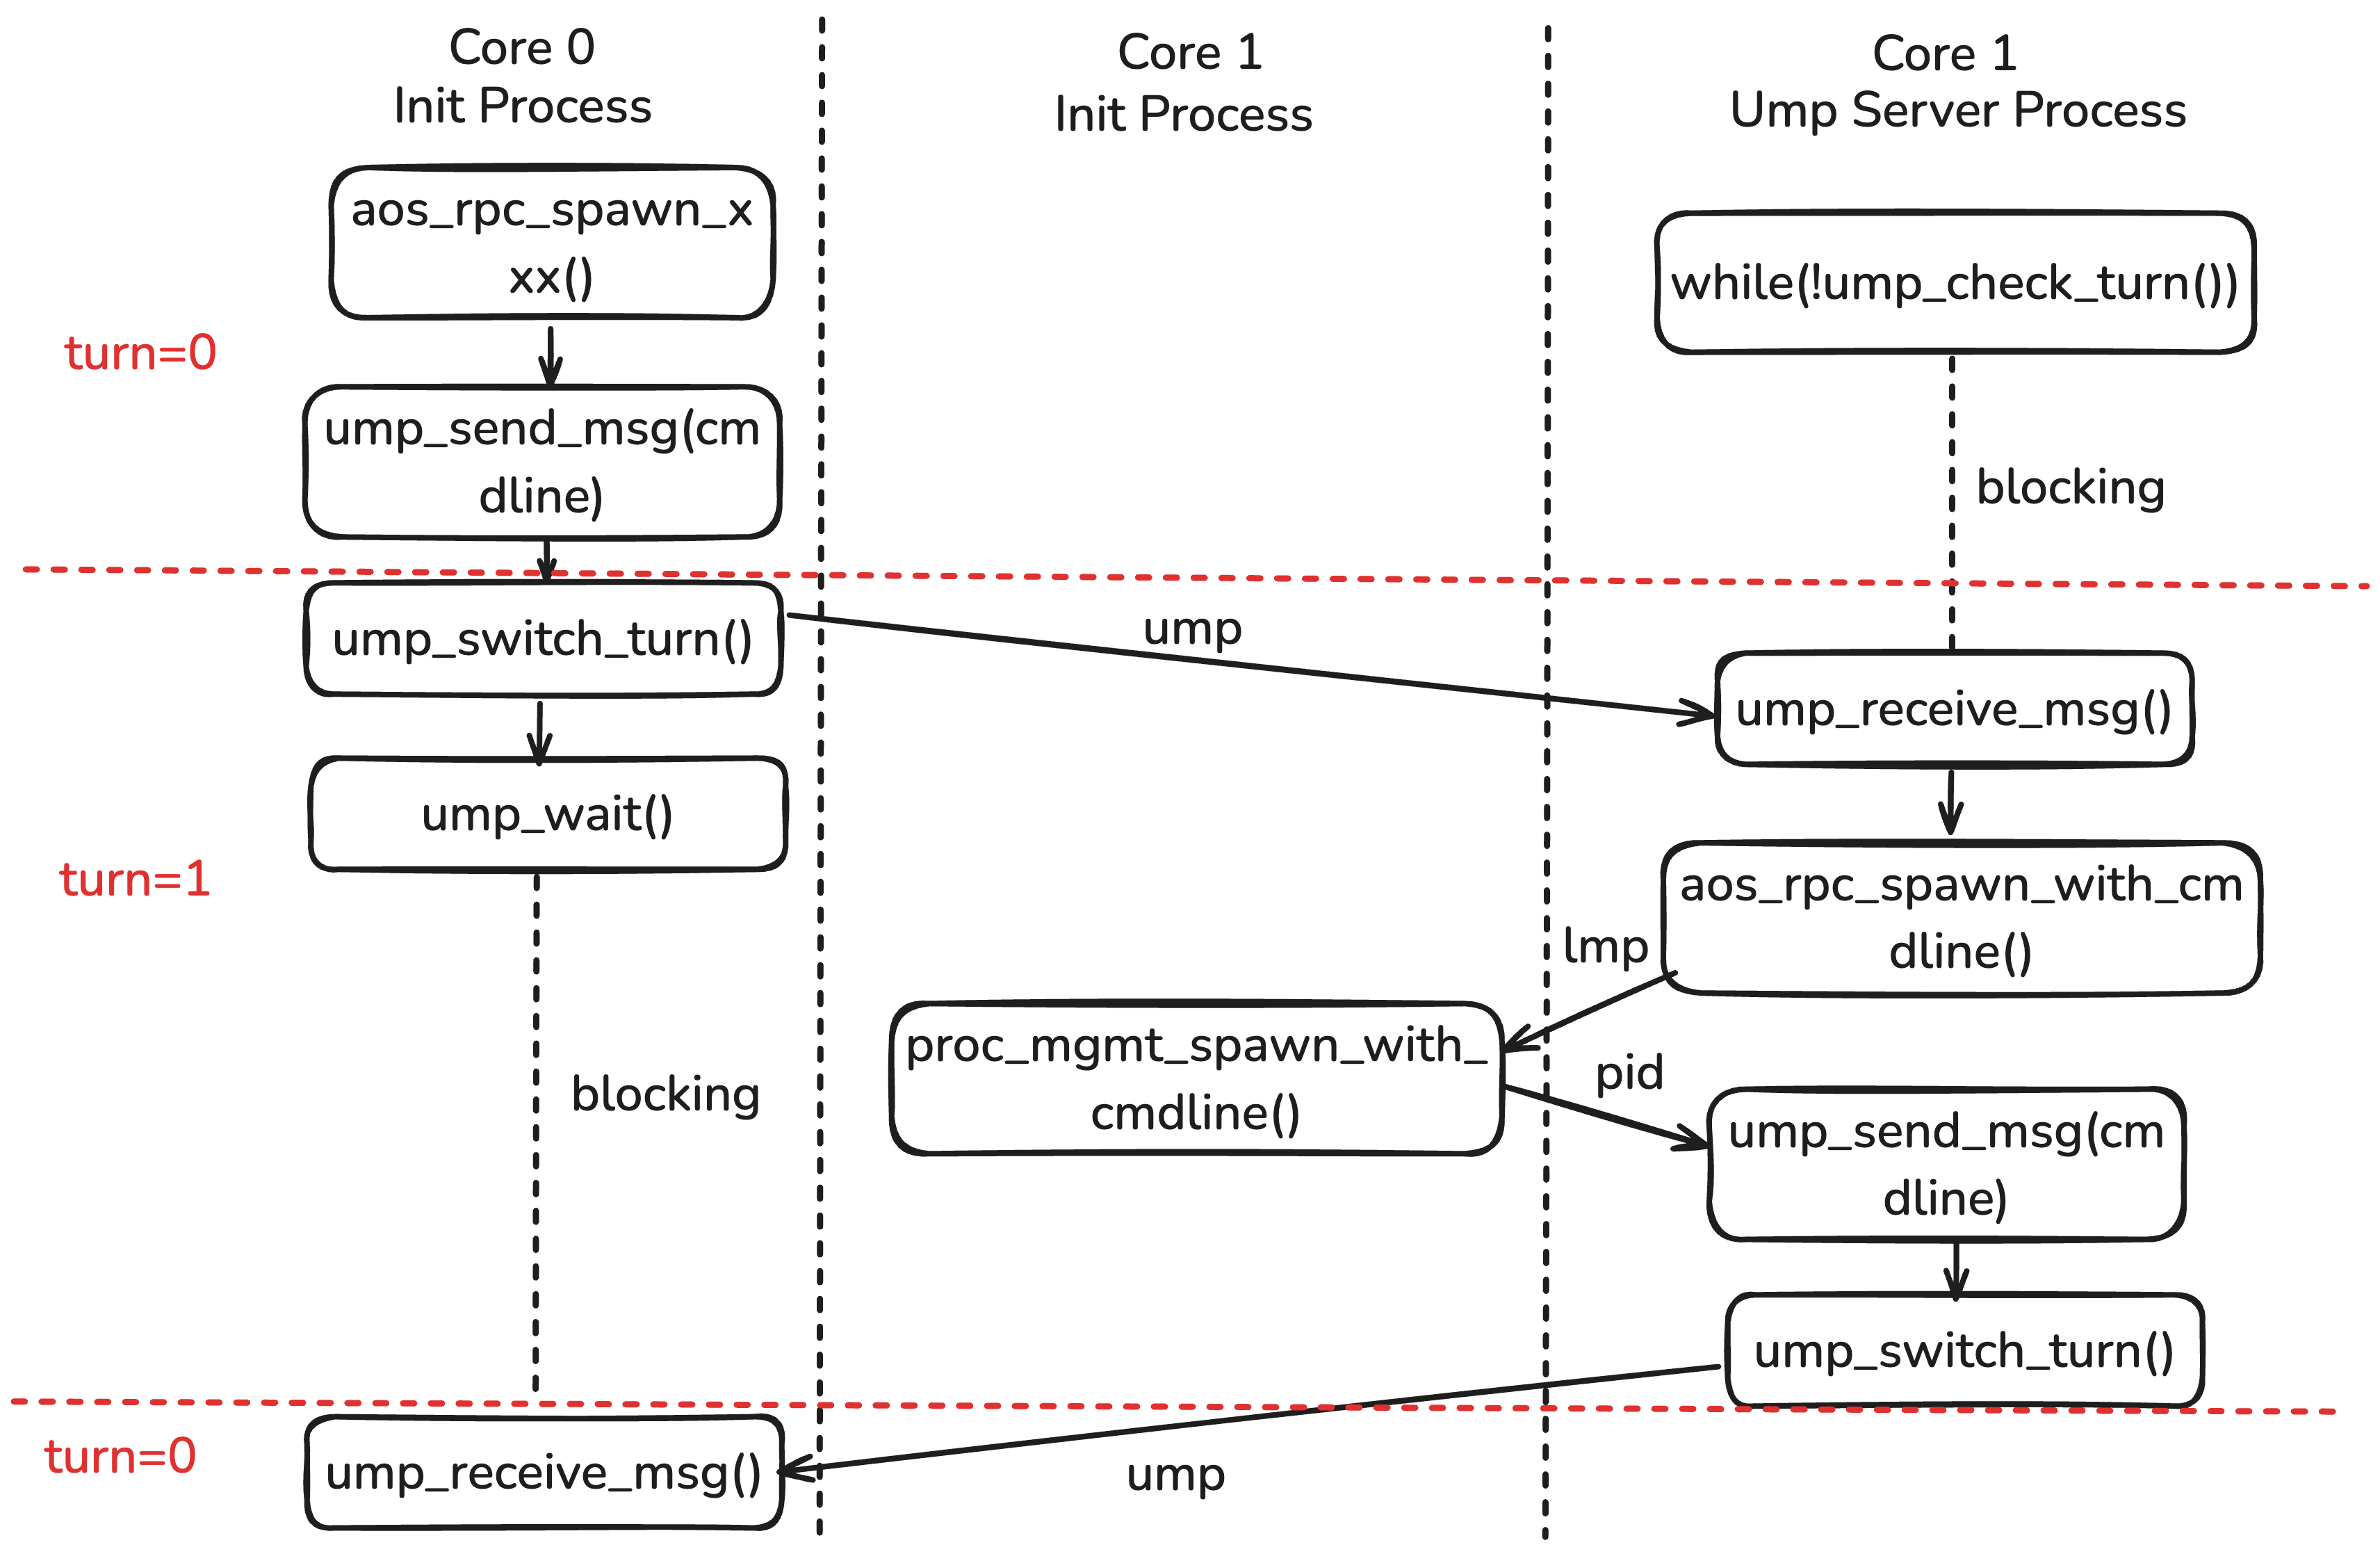
\includegraphics[width=\columnwidth]{report/images/m5-graph.png}
	\caption{Call graph outlining the steps that take place when a request to spawn a process is made across cores}
	\label{figure:spawn-call-graph}
	\centering
\end{figure}

\subsubsection*{Further Challenges} \label{sec:m5_chals}
Since we had no waitsets to rely on, our implementation diverged quite heavily from the event driven nature of our previous code. The ability to register a callback made reasoning about LMP communication quite simple, but in our M5 implementation we had to manually handle each message at time of receipt. This didn't fit well with the RPC interface and caused more holes to be punched.

Similarly, to get our unidirectional channel to function we had made many assumptions about communication. These compounded on those we'd made in M4, coming back to bite us in the implementation of M6. 
